\section{Wettkampfanalyse}

%auch die wurde weggelassen, vieleicht wenige Worte dazu verlieren
%\begin{frame}
%	\frametitle{Homologation}
%	
%\end{frame}

\begin{frame}
	\frametitle{Schweizermeisterschaft}
	
	\vspace{-3em}
	
	\begin{columns}[t]
		\begin{column}{0.45\textwidth}
			\begin{center}
				\begin{itemize}
					\item 14 Teams (12 Schweizer Teams)
					\item Probleme: ungenaues Fahren, Programmfehler, defektes Rad
					\item 4 Rang erreicht $\rightarrow$ Qualifikation
				\end{itemize}
			\end{center}
		\end{column}
		\begin{column}{0.55\textwidth}
			\begin{figure}
				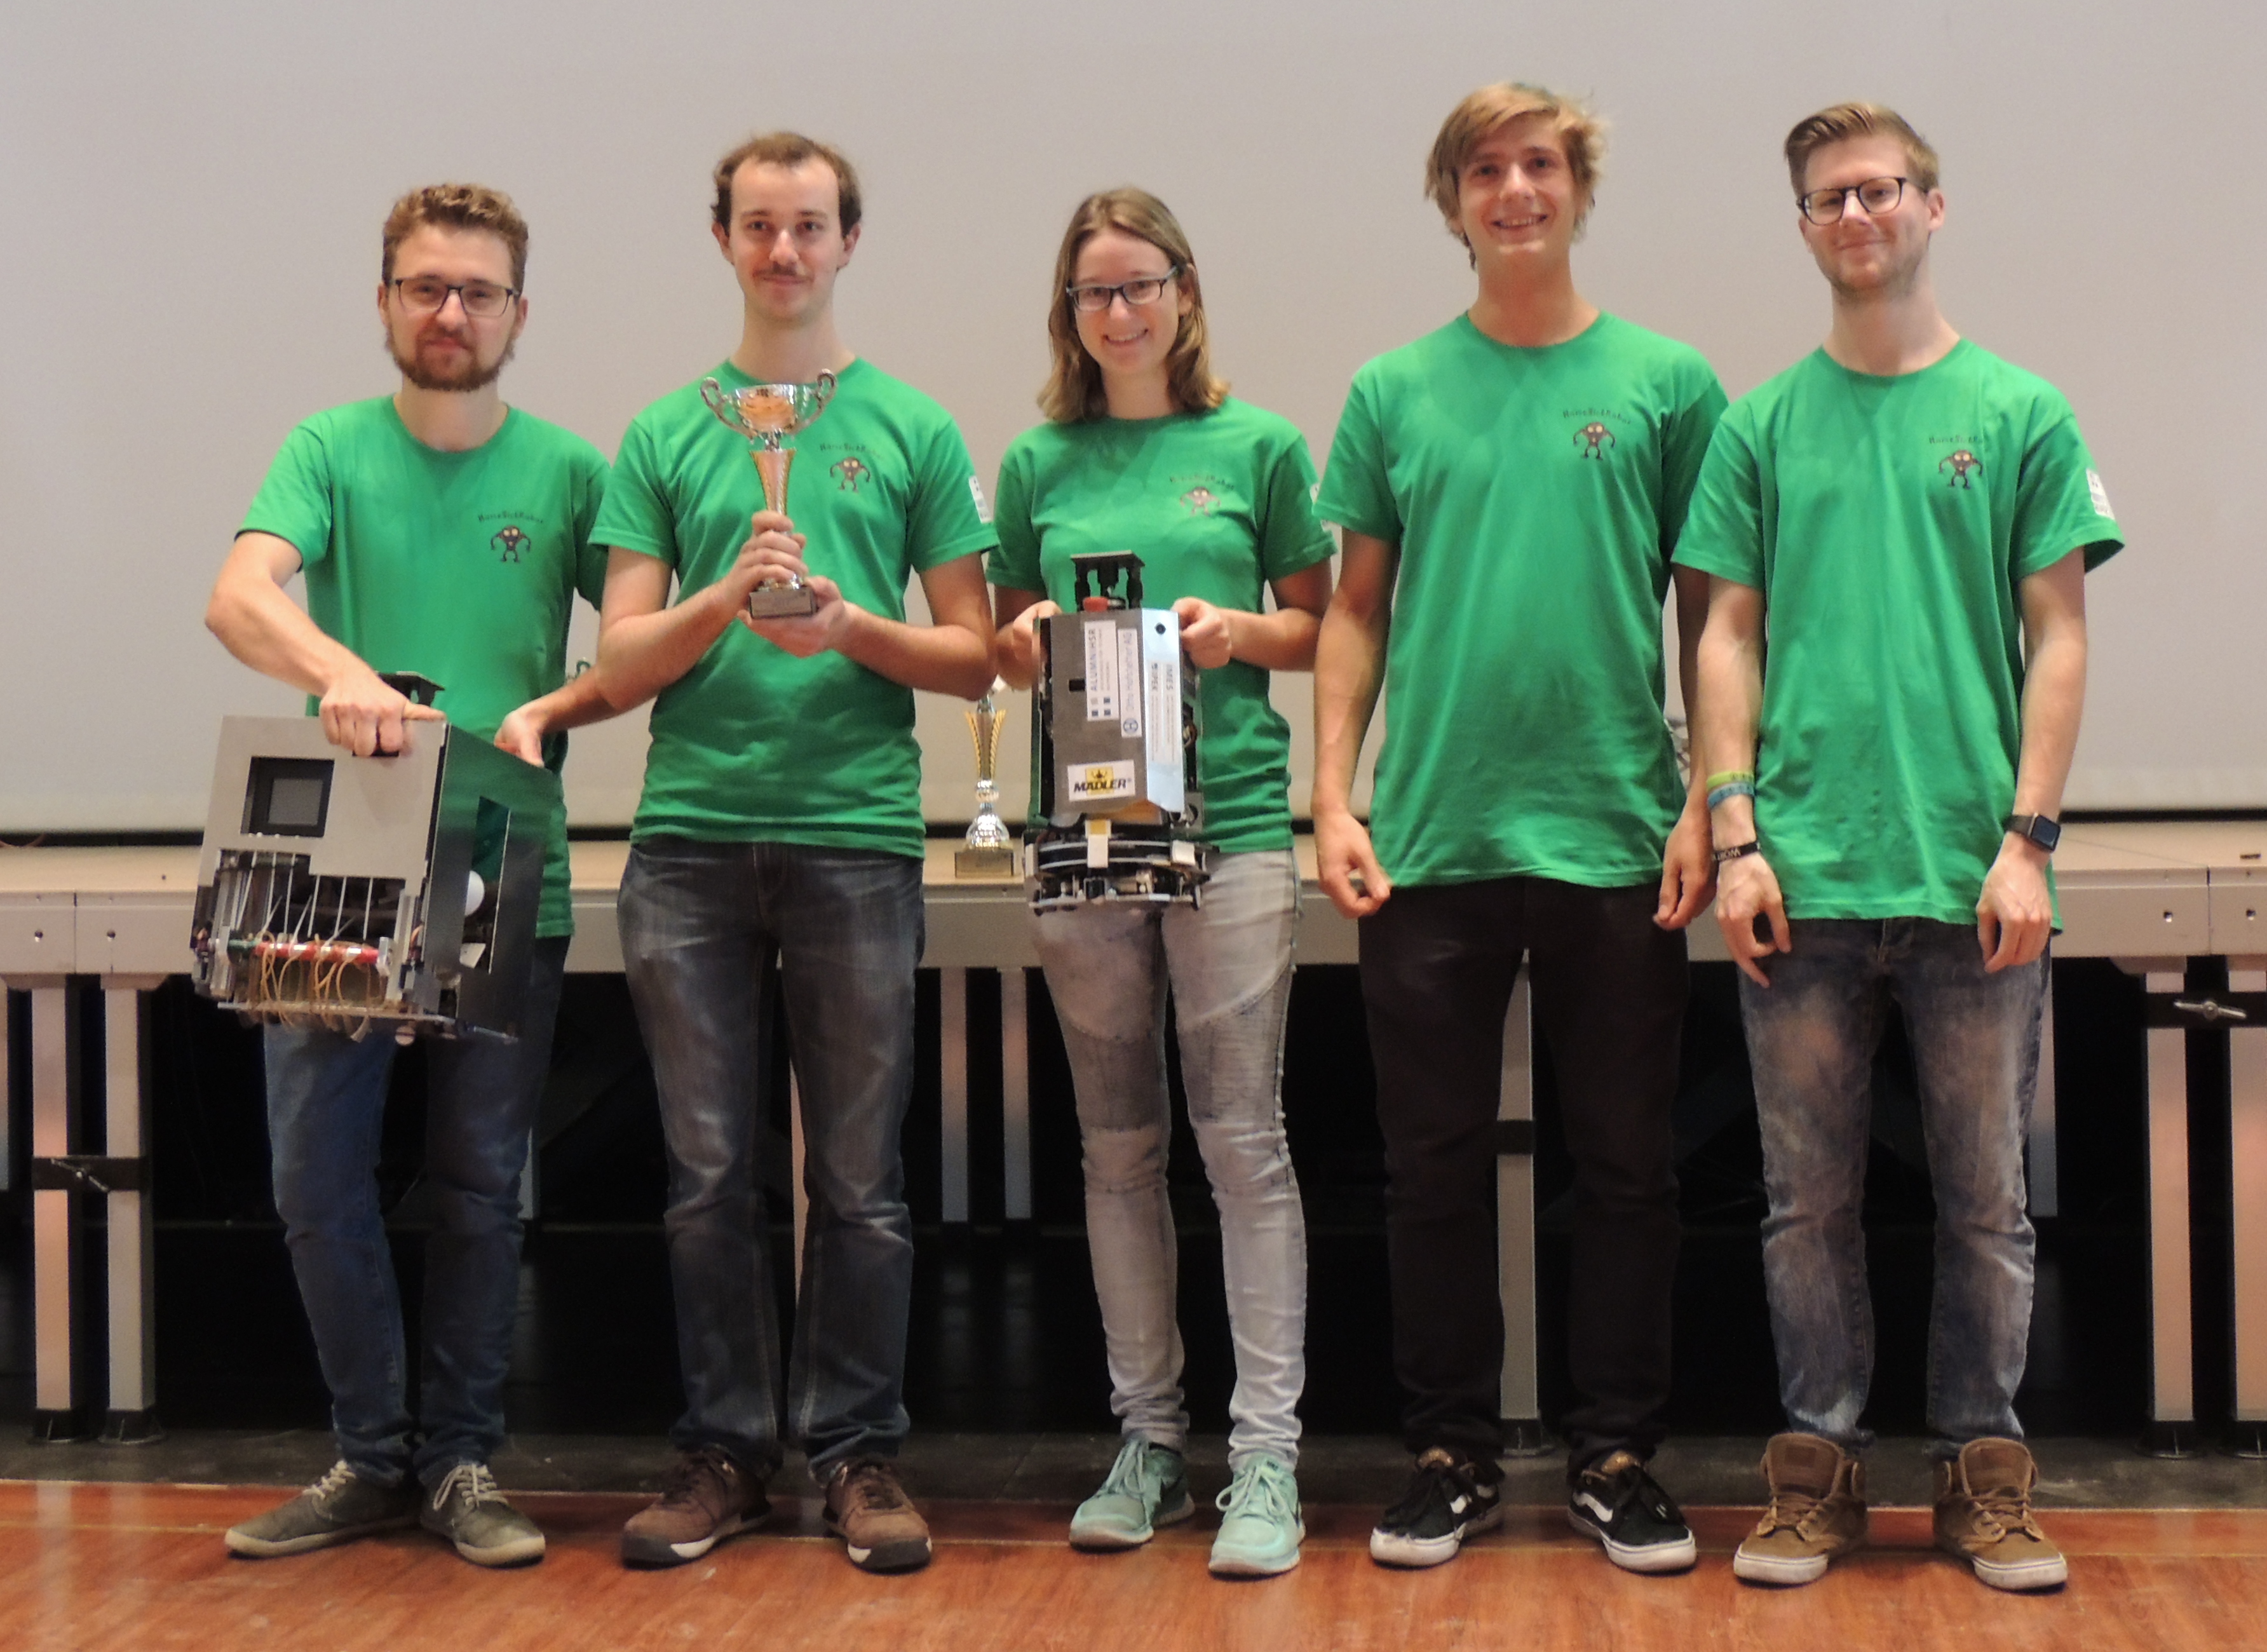
\includegraphics[width=0.9\columnwidth]{../images/presentation/swisseurobot.jpg}
			\end{figure}
		\end{column}
	\end{columns}
	
\end{frame}

\begin{frame}
	\frametitle{Internationale Meisterschaft}
	
	\vspace{-3em}
	
	\begin{columns}[t]
		\begin{column}{0.45\textwidth}
			\begin{center}
				\begin{itemize}
					\item 28 Teams (3 besten Teams aus jedem Land)
					\item Probleme: Klima (Klebband), Ungenauigkeiten des Spieltisches
					\item Viertelfinale erreicht $\rightarrow$ 8. Platz
				\end{itemize}
			\end{center}
		\end{column}
		\begin{column}{0.55\textwidth}
			\begin{figure}
				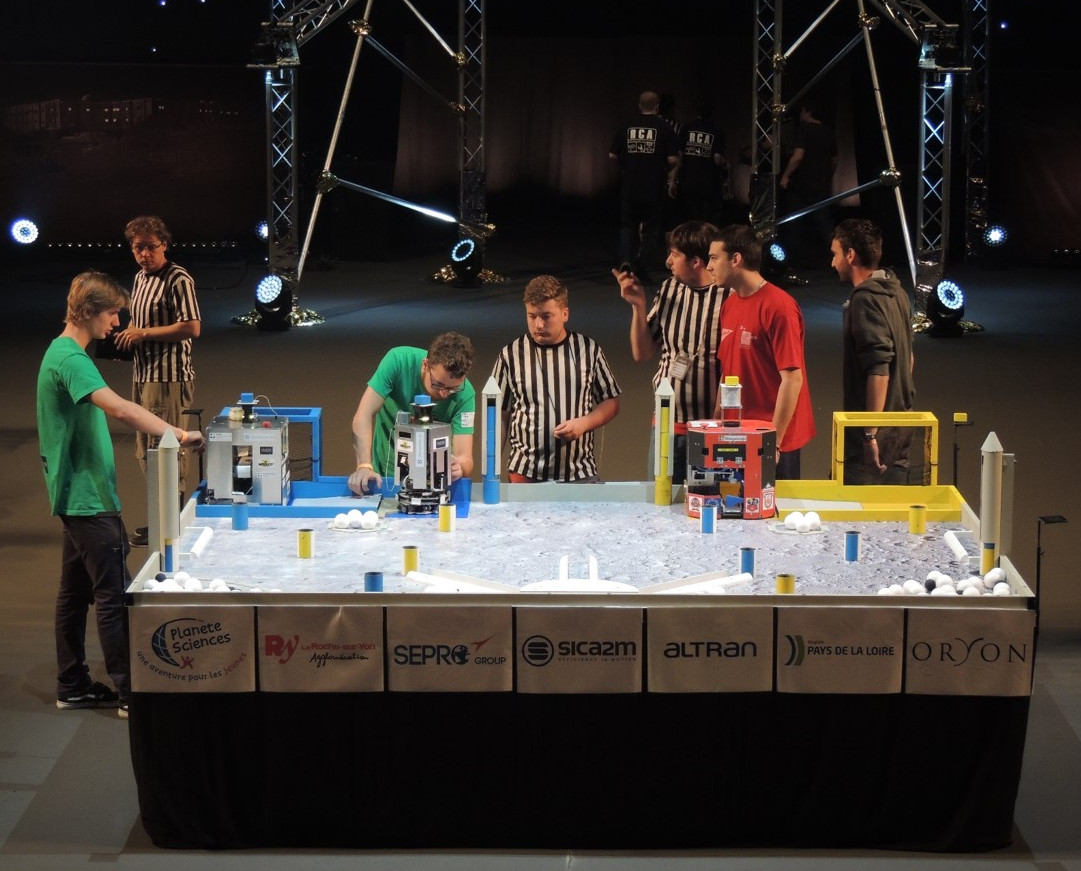
\includegraphics[width=0.9\columnwidth]{../images/presentation/international.jpg}
			\end{figure}
		\end{column}
	\end{columns}
	
\end{frame}